
\section{Introduction}
Imagine that six months ago your team decided to adopt \quotes{team code ownership.} You have enjoyed the freedom to be able to change any part of the code base. You recall that as you were implementing a feature, you found an unreported bug and simply fixed it. In fact, fixing it was easier than creating a ticket and asking the former owner to change it. Just last week, you refactored a pattern that spanned the entire system without needing to coordinate a team meeting in order to get everyone on the same page. Yet, something does not feel quite right: you literally shuddered when you looked at the Service Manager for all of its complexity and obtuse code. The creator of the Service Manager was smart, maybe too smart, but not smart enough to simplify the design. Unfortunately, the creator left the company a few months back.  While your team is permitted to modify every part of the code, you realize that you are unable to do so. Worse yet, is the underlying feeling that your team doesn't have the ability to change certain parts of the system and so cannot \quotes{own} all the code.

Shifting from individual to team code ownership is not simple; it requires multiple and complementary practices which enable a team to actively remove knowledge silos. For example, instead of strong code ownership where one developer implements a complex feature, many developers can now shape its implementation as the baton of development rotates through the team. 

%The theory of sustainable software development through team code ownership \cite{SustainableSoftwareDevelopment} introduced a solution to the problem of handling disruptions such as vacations, rotation of team members, churn, and growing team size. The theory fosters cross-sharing knowledge and simplifying code to make it easy to maintain. The theory is composed of six synergistic practices: Pair Programming, Overlapping Pair Rotation, Knowledge Pollination, Test Driven Development / Behavior Driven Development, Continuous Refactoring, and Live on Master. These practices work when the business adopts three policies: Shared Schedule, Avoid Technical Debt, and Team Code Ownership.

%The sustainable software development theory requires a shift from individual code ownership to team code ownership. Instead of strong code ownership, where one developer implements a complex feature, many developers shape the implementation of a feature as the baton of development is rotated through the team. 

At Pivotal, we observed situations affecting a team's sense of ownership which led us to the research question, \quotes{What affects the team's sense of ownership?} We relied upon constructivist grounded theory to inductively generate the categories for ownership. We collected empirical data from participant observations of an Extreme Programming project at Pivotal and through interviews of Pivotal engineers, interaction designers, and product managers.  %\strikeout{We collected additional sampling to identify which situations which would impact a programmer's sense of ownership and to identify which practices were required to enable team code ownership. }

\strikeout{In section \ref{RelatedWork}, we position the research relative to existing literature regarding team code ownership. Section \ref{ResearchMethod} describes our use of Grounded Theory. In section \ref{ResearchContext}, we present the research context by explaining Pivotal's background. In section \ref{CollectiveCodeOwnership}, we examine the factors affecting team code ownership. In section \ref{Transitioning}, we examine nuanced issues of transitioning to team code ownership. In section \ref{TheoryEvaluation}, we evaluate the theory using established criteria for evaluating a grounded theory. In the last sections, we examine threats to research validity, future research, and conclude the research.}
\section{Related Work}
\label{RelatedWork}
In Extreme Programming \cite{ExtremeProgramming2004}, Kent Beck describes a set of interdependent practices that manage feature development (much like Scrum \cite{Scrum}), as well as technical practices that facilitate a collaborative team environment. 

%\strikeout{He describes the philosophy of caretaking the code:  \quotes{In XP, everybody takes responsibility for the whole of the system. Not everyone knows every part equally well, although everyone knows something about every part. If a pair is working and they see an opportunity to improve the code, they go ahead and improve it if it makes their life easier.} } 

Kent Beck succinctly summarizes the \textbf{collective ownership} practice as \quotes{Anyone can change any piece of code in the system at any time.} \cite{ExtremeProgramming2000} He contrasts Collective Ownership against \quotes{no ownership} and \quotes{individual ownership.} In 2004, he renamed Collective Ownership to Shared Code \cite{ExtremeProgramming2004}.

In 2006, Martin Fowler defined \textbf{collective code ownership}, similarly to Beck \cite{FowlerCodeOwnership}, as a contrasting team position to \quotes{strong code ownership} where one person owns each file and \quotes{weak code ownership} where developers can change files, but an owner keeps an eye on files for which they are responsible. 

In 2011, Christian Bird et al \cite{BirdDontTouchMyCode} contrasted the effects of strong- and weak-ownership. They demonstrated that weak ownership leads to more defects than strong ownership for Windows Vista and Windows 7. The study defined ownership for a software component as a percentage of the version control commits for a single developer. They defined a major contributor as someone who has more than 5\% of the git commits. A sensitivity analysis revealed that defining strong code ownership as a range from 2\% to 10\% produced similar results for the study.

In 2015, Brendan Murphy stated that the concept of code ownership must be unpacked and expanded. He argued that the complexities of code ownership are missed by merely examining git commits to determine who modified which files. \cite{MurphyIEEESoftware}.

This paper renames \textbf{collective code ownership} to \textbf{team code ownership}. For small systems and teams, these terms are synonymous. For a large system with multiple teams, in practice, teams would have strong ownership of their portion of the system. The idea that any pair could modify any part of Microsoft Windows or Pivotal Cloud Foundry is impractical.

Team Code Ownership requires more than a team saying, \quotes{everyone can modify anything.} Instead, this paper examines how a team feels that they own the code. We define \quotes{sense of team code ownership} as the degree to which individual members of the team feel collective ownership.  

\subsection{Psychological Ownership}
Pierce et al. describe psychological ownership as \quotes{the feeling of possessiveness and of being psychologically tied to an object} \cite{Pierce2001}. Targets of ownership, whether physical or immaterial, become the extension of one's self. \quotes{what is mine becomes (in my feelings) part of ME} \cite{Isaacs1933}. Ownership can be attached to a part or the whole. Psychological ownership occurs when the object becomes part of the psychological owner's identity. Psychological ownership answers the question, \quotes{What do I feel is mine?}

Changes in ownership can have strong affects on our self-identity. An augment in possessions can produce positive effects \cite{Formanek1994}, while a diminish can lead to a personality shrinkage \cite{James1890}. Someone threatening a person's ownership can trigger strong emotions and responses.

Peirce identifies three sources or \quotes{roots} of psychological ownership: efficacy and effectance, self-identity, and having a place. A major reason for possession of physical goods or abstract ideas is rooted in the innate human desire to be in control; being able to alter one's environment creates feelings of efficacy and pleasure. Ownership fulfills the need for self-identification as people define themselves, express themselves, and ensure their own survival by what they own. Ownership fulfills the need to have a place and a territory to possess. \quotes{Each motive facilitates the development of psychological ownership, rather than directly causes this state to occur.} Psychological ownership occurs with code because creating software can satisfy the desire for efficacy and effectance, self-identity, and having a place.

Peirce identifies three paths or \quotes{routes} to ownership: controlling the target, coming to intimately know the target, and investing the self into the target. With \emphasis{controlling the target}, targets that can be controlled are perceived to be part of the self.  As  individuals repeatedly exercise control of an object, eventually this leads to \quotes{feelings of ownership toward that object.} The higher the autonomy of the job task, the more likely ownership develops toward the activity. When a person has little control over an activity, psychological ownership is unlikely to develop. With \emphasis{coming to intimately know the target}, the association with the object creates feelings of ownership. One example is when a gardener feels that the garden belongs to the gardener. (This happens routinely with software developers who feel that they own part of the code base, when in reality, the company owns the software.) Feelings of ownership increase as one becomes intimately familiar with the object and associated with it. With \quotes{investing the self into the target,} we feel that we own what we create, shape or produce. Spending time, energy, and effort enables us to alter our view of ourselves to include identity with the object. The more investing in the object, the stronger the psychological ownership. Nonroutine, complex jobs infuse more of our own ideas resulting in increased ownership.

With high ownership
- feel the right to information
— feel the right to participate in decision making
- feel responsible for it (care, protect, sacrifice for it)
-support changes that are self-initiated, evolutionary, and additive \cite{Dirks1996}
-oppose changes that are imposed, revolutionary, and subtractive
-can result in overly possessive 
- can resist in sharing ownership (overly possessive, not wanting to empower others.)





\section{Research Method: Grounded Theory}
\label{ResearchMethod}

We followed Charmaz' approach to Grounded Theory \cite{Charmaz} which provides an iterative approach to data collection, data coding, and analysis resulting in an emergent theory. The two primary data sources were field notes collected during continuous participant observations of a 7.5 month project and interviews with 21 Pivotal software engineers, interaction designers, and product managers. Interviews were recorded, transcribed, coded, and analyzed using constant comparison. 

A lengthy description of our application of Grounded Theory appears in our Sustainable So \cite{SustainableSoftwareDevelopment}.

%Grounded Theory immerses the researcher within the context of the research subject from the point of view of the participants. As the research progresses, Grounded Theory allows the researcher to \quotes{incrementally direct the data collection and theoretical ideas.} The theory provides a starting place for inquiry, not a specific goal known at the beginning of the research. As we interact with the data, the data influences how we progress and alters the research direction. 

When starting a grounded theory research study, the core question is \quotes{What is happening here?}' (Glaser, 1978) \cite{GlaserTheoreticalSensitivity}. Our initial core question was: \quotes{What is happening at Pivotal when it comes to software development?} This question led to the Theory of Sustainable Software Development summarized in section \ref{SustainableSoftwareDevelopmentTheory}. When team code ownership emerged as one of the core categories of the theory, the researcher collected additional data in order to identify the factors affecting the sense of code ownership. These factors are introduced in section \ref{TeamCodeOwnership} and are the main contributions of the paper.
\subsection{Data Collection}
The primary researcher relied on \quotes{intensive interviews} which Charmaz summarizes as \quotes{open-ended yet directed, shaped yet emergent, and paced yet unrestricted} \cite{Charmaz}. The technique relies on open-ended questions. The purpose is for the researcher to enter into the participant's personal perspective within the context of the research question. 

While exploring new emergent core categories, whenever possible, the researcher initiated subsequent interviews with a goal of not forcing the issue. For example, ``please draw your feelings about the code" often resulted in conversations about code ownership. After the interview, the interview was transcribed into a Word document with timecode stamps for each segment.

The primary researcher also collected field notes while working as an engineer. The field notes comprise of multiple paragraph entries recorded several times a week collected over a six month period. The field notes describe individual and collective actions, captures what participants defined as interesting or problematic, and include anecdotes and observations. 

\section{Research Context: Pivotal}
\label{ResearchContext}
Pivotal is a large American company with 16 offices around the world. One of its divisions is Pivotal Labs. Pivotal Lab's mission is to both deliver highly-crafted software products and provide a transformative experience for their client's engineering cultures. In order to change a developer's way of working, Pivotal combines the client's software engineers with Pivotal's engineers at a Pivotal office where they can experience Extreme Programming in an environment conducive for agile development. For startups, Pivotal might be the first engineers working on the project. For enterprise clients, Pivotal provides additional engineering resources to accomplish new business goals. 

Common team sizes are six developers plus an interaction designer and a product manager. In the history of the Palo Alto office, the number of developers on a project ranges from 2 to 28. Larger projects are organized into smaller coordinating teams with one product manager per team and one or two interaction designers per team.

Commonly utilized technologies include Angular, Android, backbone, iOS, Java, Rails, React, and Spring often deployed onto Pivotal's Cloud Foundry. 

Pivotal Labs has followed Extreme Programming \cite{ExtremeProgramming2004} since the late 1990's. While each team is autonomous in making its own decisions as to what is best for a particular project, the company culture strongly suggests following all of the core practices of Extreme Programming. This includes Pair Programming, Test Driven Development, Weekly Retrospectives, Daily Stand-ups, Prioritized Backlog, Whole Team ownership of the project and code base, plus Kanban's notion of work flowing through people.


\begin{table*}[t]
\renewcommand{\arraystretch}{1.5}
\centering
\caption{Theory of Sustainable Software Development: Principles, Policies, and Practices}
\label{SustainableSoftwareDevelopmentTable}
\begin{tabular}{|p{1.65in}|p{1.35in}|p{1.8in}|p{1.6in}|}
\hline
\multicolumn{4}{|c|}{Sustainable Software Development}                     \\
\hline
Underlying Principles & Policies                  & Removing Knowledge Silos Practices & Caretaking the Code Practices       \\
$\bullet$ Keeping a Positive Attitude Toward Team Disruption & $\bullet$ Team Code Ownership & $\bullet$ Continuous Pair Programming         & $\bullet$  TDD / BDD                   \\
$\bullet$ Encouraging Knowledge Sharing and Continuity & $\bullet$ Shared Schedule           & $\bullet$ Overlapping Pair Rotation & $\bullet$ Continuous Refactoring      \\
$\bullet$ Caring about Code Quality  & $\bullet$ Avoid Technical Debt      & $\bullet$  Knowledge Pollination    & Supported by Live on Master \\ 
\hline
\end{tabular}
\end{table*}


\section{Theory of Sustainable Software Development}
\label{SustainableSoftwareDevelopmentTheory}
The Theory of Sustainable Software Development through Team Code Ownership is fully presented in \cite{SustainableSoftwareDevelopment}, summarized in this section, and illustrated in Table \ref{SustainableSoftwareDevelopmentTable}. The theory describes how teams can continue to deliver value in spite of team disruptions. The theory is a collection of synergistic principles, policies, and practices encouraging a positive attitude towards team disruption, knowledge sharing and continuity, as well as caring about code quality. 

\subsection{Principles}
The theory underlying principles are as follows: \textbf{Keep a Positive Attitude Toward Team Disruption} by recognizing the value that new team members bring with their fresh perspectives and challenging team assumptions; \textbf{Encourage Knowledge Sharing and Continuity} by enabling the knowledge to spread from one developer to the next, and eventually, reach the entire team; and \textbf{Care about Code Quality} by recognizing that a well cared for code base makes modifications easier. 

\subsection{Policies}
\textbf{Team Code Ownership} empowers engineers to modify any part of the system under the team's responsibility. When engineers agree that a section of the system needs to be changed, the team proactively and tacitly authorizes the change. \textbf{Shared Schedule} aligns the team's work schedule to enable efficient daily rotation of the developers working on a track of feature development. \textbf{Avoid Technical Debt} enables a team to balance feature development with Continuous Refactoring. When a team is pressured to finish work by a deadline, it might be tempted to focus on feature delivery, stop refactoring, and hence take on technical debt. The team should prefer consistent software development by caretaking the code and leaving the code base in a state where any member of the team can pick up the next story for that part of the code base. This requires product and management support to avoid unnecessary thrashing of developers rushing incomplete work by taking on technical debt in order to deliver a feature early.

\subsection{Removing Knowledge Silos Practices}
By sharing knowledge throughout a team, any pair will have enough context to understand what needs to be done and know who to ask if they need more details. \textbf{Continuous Pair Programming} reinforces that there is no single owner for any line of written code. The team owns the code. As two developers collaborate, they generate shared context. That knowledge will spread around the team the following day via \textbf{Overlapping Pair Rotation} which explicitly rotates people off a track of work in order to cross-pollinate knowledge and avoid emergent knowledge silos and individual ownership. \textbf{Knowledge Pollination} is activities that promote knowledge sharing in unstructured ways between pairs and includes activities such as daily stand-ups, writing on whiteboards, overhearing a conversation, calling out an update to the team, or simply reaching out to others to ask questions as needed. 

\subsection{Caretaking the Code Practices}
By caretaking the code, the team enables any pair to be able to work on any story in the backlog.  \textbf{Test Driven Development (TDD) / Behavior Driven Development (BDD)} creates a safety net of tests that give any pair the courage to modify the system without the fear of breaking some other part of the system unexpectedly. The tests become a specification on how each component is used. \textbf{Continuous Refactoring} increases code quality by increasing code discoverability (knowing where to find the responsible code), increasing code readability, and increasing the simplicity of design.  \textbf{Live on Master} enables the team to perform Continuous Refactoring as the code is easy to integrate. When teams have long running development branches, merge conflicts discourage Continuous Refactoring. 

%\subsubsection{Pair Programming}
%When each line of code is written by two developers, there is no clear owner. The pair can develop a shared sense of ownership over the code that they both contributed.

%\subsubsection{Overlapping Pair Rotation}
%Overlapping Pair Rotation is the daily rotation of half of the pair on each track of work. The rotation of developers breaks down knowledge silos and spreads context throughout the team. In a short time, individuals will work on multiple parts of the system. 

%Here is an example pairing rotation for a four person team: \texttt{
% Day 1: (A B), (C D)
% Day 2: (A C), (B D)
% Day 3: (A D), (B C)
% } On a four person team, the new pairs have full context about yesterday's changes, which ensures confidence.

%In some extreme programming companies, pairs never rotate. Two people work on one part of the code base, developing strong ownership. The rest of the team does not feel empowered to modify their code as they rarely work on it. 

%\subsubsection{Continuous Refactoring}
%Most stories typically involve some refactoring. Developers are encouraged to refactor in order to make the code's design cleaner, to improve reuse by making the code easier to understand, and improve clarity by making it easier to find associated components.  Usually, the team prefers \quotes{pre-factoring} where the developer does the complicated work to make the implementation of the current story as simple and easy as possible, as oppose to \quotes{post-factoring} where refactoring happens after the story is done, but before it is delivered.  Sometimes it is hard to anticipate refactorings, in this case just implement the story, and refactor out duplication.

\begin{table}[]
\renewcommand{\arraystretch}{1.5}
\centering
\caption{Factors affecting Team Code Ownership}
\label{TeamCodeOwnerhipFactors}
\begin{tabular}{|p{3.1in}|}
\hline
System Context Level \\
Code Contribution Level \\
Code Quality \\
Product Quality \\
Team Belonging Level \\
\hline
\end{tabular}
\end{table}

\section{Team Code Ownership}
\label{TeamCodeOwnership}

In the literature, collective code ownership is often treated as a policy statement. In practice, a team claiming that \quotes{anyone can modify any piece the code} is not sufficient to achieve the desired results. The theory of sustainable software development presented in the previous section introduces a set of synergic principles, policies, and practices that must be in place to achieve team code ownership. 

The sense of team code ownership is a spectrum. On one side, each individual has ownership of only their code;  on the other side, everyone on the team owns the entire code base. A team striving for team code ownership may land somewhere in between. 

Our research revealed that the sense of team code ownership is dynamic. Negative project influences can erode the team's sense of ownership over the project's duration. A team needs to counteract these erosions in order to increase their sense of ownership. Ownership is an emotional or qualitative attribute which ties all developers on the team to the project and code base. Our research question is the following:

\textbf{Research Question:} What are the factors affecting the sense of team code ownership?

We identified five factors listed in Table \ref{TeamCodeOwnerhipFactors} that affect the team's sense of ownership over a project's duration: system context level (\quotes{how much do I know about the code and the system}), code contribution level (\quotes{how much have I contributed to the code}), code quality (\quotes{how confident am I about the code quality}), product quality (\quotes{how confident am I about the product quality}), and team belonging (\quotes{how connected am I to the team.})

\subsection{System Context Level}
\textbf{Definition:} Context is the knowledge and situational awareness about the code, including the discourse that surrounds the code. Context includes  understanding how existing features have been implemented, understanding existing design decisions, understanding underlying technologies and frameworks, and understanding how features solve the user's need.

\textbf{Purpose:} Developing a deep knowledge of the system exercises the \quotes{intimately knowing the target} path of psychological ownership.

For a pair to be able to work efficiently on any part of the system, one of them needs to have enough context to know how that part of the system works. Without enough context, a pair might struggle, slow down, or be blocked in working on a feature. If this happens, the team could re-rotate pairs for that day and the team should examine for an emerging knowledge silo. 

Code ownership seems to vary with the context that the developer has about the code; the more the developer knows, the higher the sense of ownership. The size of the code base or the number of developers working in parallel can make it difficult for a programmer to develop a deep system context level.

\textbf{Threat: Increasing code base size.} The primary researcher participated on a team working with a large code base that was over eight years old and the team did not have a full understanding of the system. Initially, the team felt little ownership of the code, even though the team was responsible for it and agreed to \singleQuote{team code ownership.} Often the team would need to ask a product manager why certain features existed in the code to understand what the code was trying to do. In time, as the team worked with the code and gained context, the team's sense of ownership improved.

\textbf{Threat: Increasing team size.} The primary researcher observed the relationship between team size and code context on five Pivotal projects as a participant-observer. As team size increases, the ability to gain system context decreases. Every day, all pairs are adding to the system. On a five pair team, so much work is happening each day that it becomes increasingly difficult to keep track of everything that changes.

One developer on a 10 person project said, \participantQuote{I feel that we don't have the context spread around fully. Having five, sometimes six, pairs on the project makes it go really fast, so it's hard to keep context.}

When developers do not have context about part of a system, or context about what remains to be done to finish a story, reluctance to start the next story at the top of the backlog emerges. It's easier to start a story that touches part of the system that they know. As one developer reflected, \participantQuote{I am not completely comfortable to jump into stories on certain aspects [of the system].}

As a coping strategy, one developer, before the start of the work day, skimmed the git commits from the previous day in order to learn about new classes and changes in design, and to understand the features the team added. As a possible mitigation strategy, each pair of the team could start their pairing day by reviewing changes from the previous day. For a large team, this additional work becomes increasingly necessary. 

As team size grows, there is a potential risk of decreasing an individual developer's sense of team code ownership. 

\subsection{Code Contribution Level}
\textbf{Definition:} Code contribution is the portion of the code that a given developer has worked on. 

\textbf{Purpose:} Personally contributing to the code base increases a developer's sense of ownership by exercising \quotes{investing in the target} path of psychological ownership. As a developer works on the code base, the developer's system context level increases. While code contribution level influences the system context level, it is not necessary related: developers might learn about the code through other means different from direct contribution, including conversations at stand-up, impromptu team huddles, or a pair saying \participantQuote{Check out what we did yesterday.}

\textbf{Threat: Inability to contribute.}  A developer's inability to contribute to the code base decreases the developer's sense of ownership. This could happen for instance during a pair programming breakdown. When the pairing experience breaks down, one person drives the code development while the partner passively watches. When one person is writing all the code, individual code ownership replaces team code ownership.  

In one situation, the partner took over and ignored the participant's input. The participant reflected, \participantQuote{I did not understand what was really going on. I wouldn't be able to explain deeply what we had done. I wouldn't be able to maintain it. I didn't really write it, so I feel very little ownership of it.} 

We call \quotes{Performance Pair Programming} when one developer plows through a story and stops listening to the developer's partner. Ideally, Pair Programming is a collaborative experience where both individuals are unable to tell who wrote which portions of the code. 

\subsection{Code Quality}
\textbf{Definition:} Code quality relates to how well the code satisfies the project's desirable quality attributes. Desirable quality attributes might include design qualities (conceptual integrity, maintainability, reusability, discoverability), run-time behavior (availability, interoperability, manageability, performance, reliability, scalability, security), system qualities (supportability, testability), and user qualities (usability) \cite{Meier2009}. 

\textbf{Purpose:} How well the code satisfies the project's desirable quality attributes affects the team's sense of ownership. When a product does not achieve an acceptable quality level, an engineer may not want to be identified with the product and thus the self-identification motivation of psychological ownership is not being met. Low quality products also tend to involve a disproportionate amount of bug fixes. Developers need a balance between creating new features and fixing bugs each week. Working only on bugs for weeks affects their sense of ownership.    

\textbf{Threat: Pressure to Deliver and Deprioritizing Continuous Refactoring.} When developers are pressured to deliver more features at the expense of Continuous Refactoring, the code acquires technical debt, the code becomes harder to work with, and developers can begin to feel apathetic about the code. When developers begin to experience code apathy, this decreases their sense of team code ownership. 

When refactoring is neglected, new code is simply bolted onto the existing design. Each time the team bolts something else on, it gets more difficult to bolt on the next piece. Thus, a dilemma arises for the programmers working on the next story that touches this part of the code: do they continue bolting on more code, or do they perform the pretermitted refactoring? When the team begins avoiding refactoring, it's a sign that code apathy may be settling in. Code apathy results in reduced quality, as the developers become less invested in the craftsmanship of the code.

One developer felt \participantQuote{proud and disgusted} about the code base. He is simultaneously proud of each refactoring that the team performed and disgusted by the technical debt the team accrued by taking shortcuts to ship more features. The developer drew Figure \ref{Programmer1} to shows their feeling about the code, \participantQuote{It is generally orderly with a few bits that maybe are not as orderly.}

Before the first launch of a product, the product manager suggested that the team deliver more features at the expense of technical debt. For some of the team, this was an unacceptable tradeoff, and those developers decided not to cut corners. Others on the team complied with the request and incurred technical debt. The entire team ended up paying the consequences with extensive refactors after the launch. On a communal code base, one pair adding tech debt affects everyone on the team.

When code apathy settles in, team members adopt the attitude that someone else will solve the problem with the code. When this attitude permeates a team, no one is solving the problems. 

\begin{figure}[t]
\centering
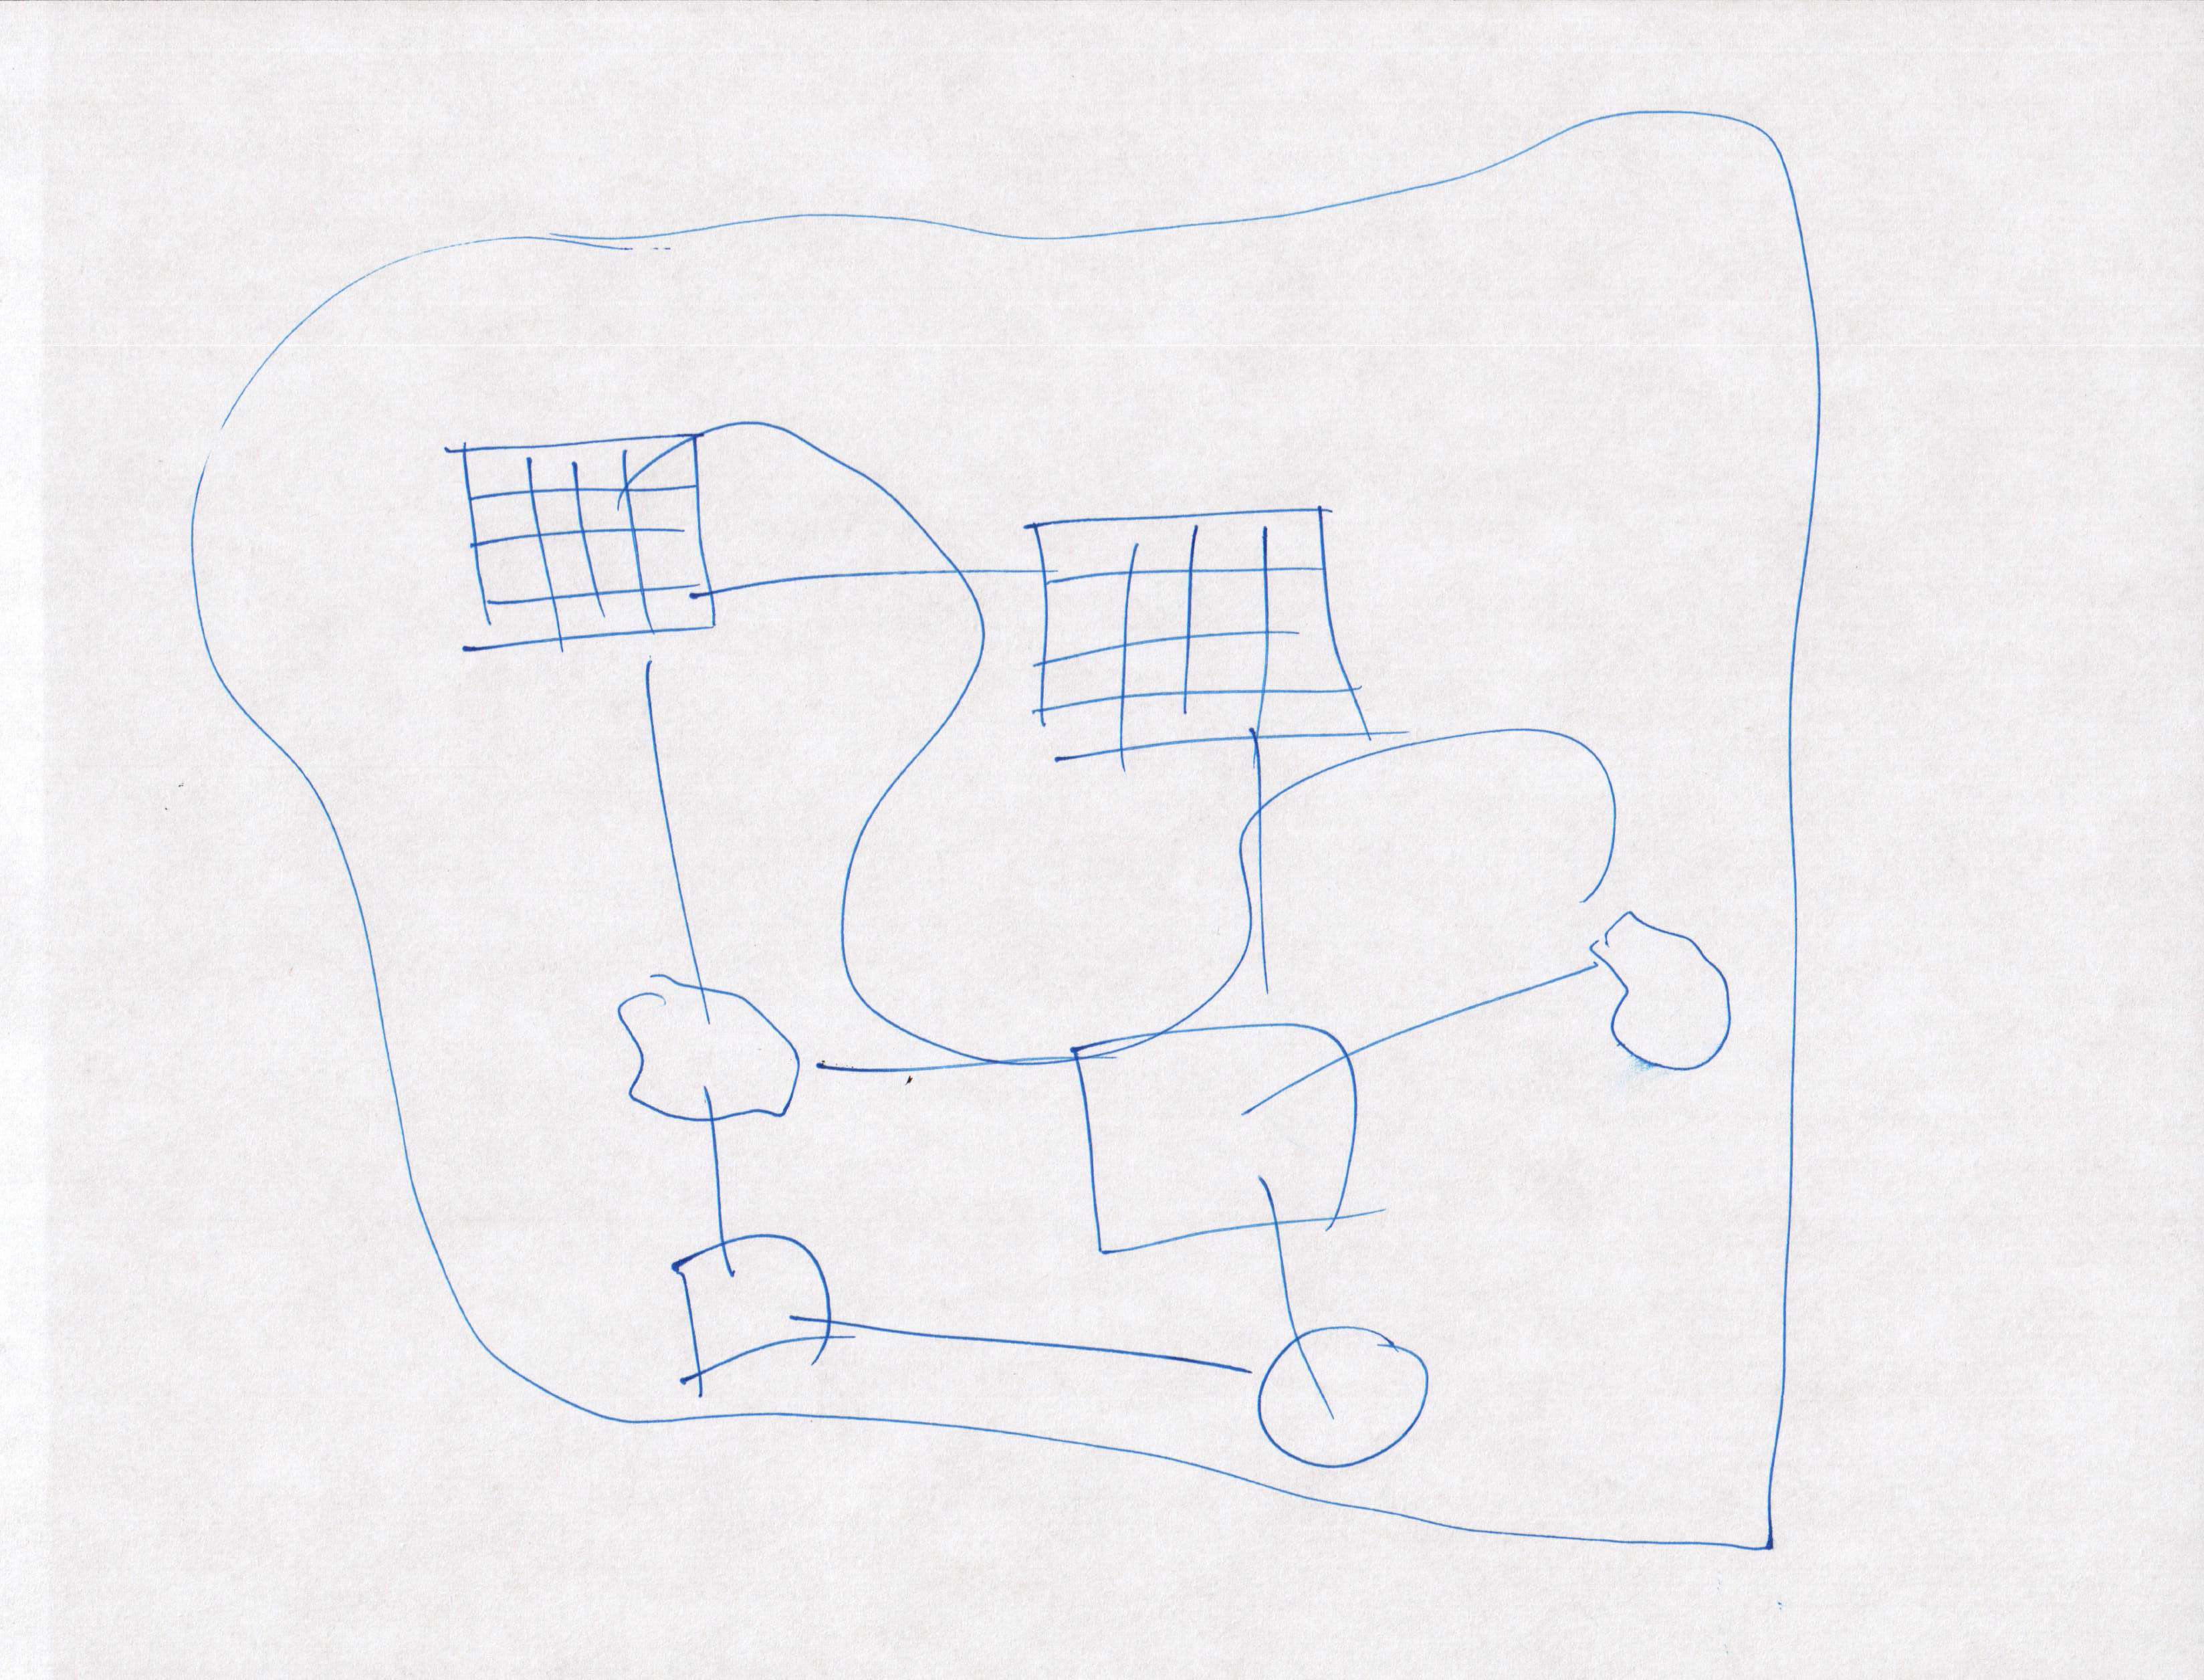
\includegraphics[width=3.45in]{CodeOwnership.jpg}
\caption{\quotes{Draw how you feel about the code}}
\label{Programmer1}
\end{figure}


The team wants to feel \quotes{pride in improving code quality.}  It feels good to be improving the code design and readability. If the team starts neglecting these concerns, it can engender a sense of disgust and an apathy for the code can spread throughout the team.

\subsection{Product Quality}
\textbf{Definition:} Product quality is believing that the product will solve the user's need.

\textbf{Purpose:} Pivotal engineers want to produce products that will matter to the user. Delivering a product that matters to someone satisfies the self-identity motivation of psychological ownership.

\textbf{Threat: increasing product apathy.} Product apathy occurs when a developer loses investment in the features of the product. Pivotal's balanced team approach is founded on collaboration. When product managers, or other stakeholders, ignore feedback from the developers, the developers can begin to feel less ownership in the product, and in turn be less motivated to work on the project.

When picking up a story, developer should verify that the story contains clear acceptance criteria. If it does not, the developer typically clarifies with the product manager what must be done. On one project when the stakeholders were ignoring feedback from the developers, one developer recalled, \participantQuote{In this case, I don't feel like spending the extra energy to go and say, `Hey, are you sure? Is this what you want?'} 

%Given the technical complexity of a product, sometimes the next story on the backlog can be blocked. Instead of proactively working with product, one developer adopted the attitude: \participantQuote{Well, this [story] is blocked and it's somebody else's problem.} 

Product apathy can result in a poorly crafted product that does not meet the customer's needs.

\subsection{Team Belonging Level}
\textbf{Definition:} Tem belonging is when team members feel part of the team and are proud of the team's accomplishments.

\textbf{Purpose:} This satisfies the \quotes{having a place} motivation of psychological ownership.

\textbf{Threat: increasing team apathy}
Team apathy manifests when developers do not feel that they are a part of the team. It is hard to feel team ownership of the code base when one feels excluded from the team.

We observed several behaviors that can distance an engineer from the team: interrupting the engineer during discussions, using poor listening skills so that the developer feels unheard, or talking beyond the engineer's level of technical expertise. 

On one team, during discussions the team talked about code but never looked at the source code. For one visual learner, it was hard for the programmer to follow the discussions. Sometimes the team discussed parts of the code that the individual had not seen recently. When the team discussed two variants of coding practices without showing concrete examples, the programmer could not contribute. When the developer raised this issue to the team and the team continued with the status quo, the programmer felt marginalized by the team.

Poor onboarding of developers can contribute to developers feeling isolated. On one project, there was a time crunch and the team was feeling the pressure to deliver stories. When the team added developers, the team had a \quotes{sink or swim} attitude. For example, one person was left alone with no clear idea on how to proceed for the first couple of hours on the project. If someone does not feel part of the team, how can they feel ownership of the code base? Making a new team member feel welcome is important.


%tmp comment to get paper into 6 pages
%As another developer expressed, \participantQuote{Not listening to each other can create apathy.}

When developers feel that the team does not care about them, their sense of ownership can decrease.
\section{Transitioning to team code ownership}
\label{Transitioning}
Since Sustainable Software Development requires a shift from individual code ownership to team code ownership, the transition should not be taken lightly. 

%Some individuals derive their sense of value, worth, and identity from what they produce. Shifting from individual code ownership to team code ownership, asks people to shift how they value and perceive themselves, and thus the transition should not be taken lightly.

The developer changes from the role of owner to the role of steward or caretaker. In one interview, a software engineer struggled to describe the developer's relationship with the code on a very challenging project and settled in on the caretaker metaphor: \participantQuote{Sometimes I kind of feel like a janitor to [the code base].  Maybe caretaker would be better. Yeah, probably caretaker. I feel like a janitor just cleans up messes, but a caretaker makes things better.}

Some developers effortlessly make the transition to team code ownership. They immediately see the benefits of being able to modify any part of the code base and quickly shift from \participantQuote{I made this} (personal ownership) to \participantQuote{we made this} (collective ownership.)

Some developers struggle with adjusting to team code ownership as they miss having a piece of code or functionality that they exclusively developed and hence recognize as their own. Some people derive their sense of value, worth, and identity, from what they produce. The transition requires people to change their relationship with what they produce and shift how they value and perceive themselves. 

A recent hire to Pivotal described his initial experience as, \participantQuote{Seeing my work slowly removed from the app,} as he witnessed his code modified, and eventually replaced, through various refactorings. When reflecting on the daily rotation, this developer recalled occasions of wanting to hang on to his work.  Over time, his attitude of \participantQuote{I want to see it through,} evolved into, \participantQuote{Someone else is going to take over and they're going to do fine. I can move onto something else and that's okay.} 

The engineer learned the rhythm of story rotation and developed trust in his team realizing that the rest of the team will do a good job. Developers rolling off a story in flight can look in anticipation to see how the next pair solved the problem. 

Eventually, team members recognize the lack of long-term individual authorship, learn to expect their code to be transitory, and thus loosely hold personal contributions. \participantQuote{The code that I write today may be in the code base for a little while, and it will evolve into something better.}  

For a developer with strong individual ownership tendencies, we recommend transitioning to team code ownership by placing this person on a four-person team. This allows the person to see the benefits of shared code ownership while slowly releasing individual ownership. On a four-person team, each daily rotation creates pairs with full knowledge of what happened yesterday.  

% Here is an example pairing rotation illustrating that each day, the new pairs have full context about yesterday's changes:
% \texttt{
% Day 1: (A B), (C D)
% Day 2: (A C), (B D)
% Day 3: (A D), (B C)
% }

One Pivotal engineer uses improvisation games and collaboration games to help teams practice letting go of control, trusting the team, and learning to be pleasantly surprised by what emerges. In this regard, sustainable software development is an ensemble performance. 

When a team achieves a sense of collective ownership, the magic happens: \participantQuote{People are a lot more flexible all across the board, with changing things or accepting feedback or collaborating,} and \participantQuote{We want the best possible product that's best for users \ldots we just want the best thing out there.} Then the team can say \participantQuote{Hey, this is our code!}

\section{Theory Evaluation}
\label{TheoryEvaluation}

In assessing a Grounded Theory research study, Charmaz identifies four criteria for evaluating a grounded theory study: credibility, (\quotes{is there sufficient data}), originality, (\quotes{do the categories offer new insights}), resonance (\quotes{does the theory make sense to participants}), usefulness (\quotes{does the theory offer useful interpretations}) \cite{StolGTinSE}. 

\textbf{credibility:}  The number of open-ended interviews and the field notes from participant observation serve as a rich data set for the analysis. 

\textbf{originality:} Team code ownership is more than a policy statement that anyone can modify any part of the code. This paper broadens the idea of team code ownership by acknowledging that many factors can affect the team's sense of code ownership.

\textbf{resonance:} When shown to participants, they resonate with the factors that affect team code ownership and understand how the threats can weaken ownership.

\textbf{usefulness:} 
The theory explains how different factors affect ownership and illustrates how team actions can influence ownership. 

\section{Threats to Validity}

\subsection{External Validity}

\textbf{Generalizability across situations:} a grounded theory limitation is that the theory emerges from a particular context and may not apply to other situations. This work analyzed software projects at the Silicon Valley office of Pivotal following Extreme Programming. The results might not apply to other teams in industry wanting team code ownership or following Extreme Programming. Replicating the results with other teams would mitigate this threat. 

\subsection{Internal Validity}
\textbf{Researcher bias:} a risk of the participant-observer technique is that the researcher may lose perspective and become biased by being a member of the team. An outside observer might see something the researcher missed. We mitigated this risk by recording interviews and with a colleague reviewing the coding process. 

\textbf{Prior knowledge bias:} with grounded theory prior knowledge can aid the researcher in looking at interesting research questions or create difficulties in blinding the researcher about possible explanations \cite{GlaserIssues}. We mitigated this risk with a colleague reviewing the coding process. 
\section{Future Research}
Developers, interaction designers, and product managers all have different goals in their roles. In future work, we plan to examine how factors for each role drives ownership.

Some programmers naturally adapt to team code ownership, while others struggle with the transition. In future research, we will follow new Pivotal engineers and examine their journey in transitioning from individual to team code ownership. This may uncover specific practices that Pivotal or the development team could employ to ease the transition. 

%temp comment to make paper fit in 6 pages
%Further research is necessary to determine the optimal team size for team code ownership. Early indications suggest that a four-person team is a optimal for introducing team code ownership. With a four-person team, each pair  is working on half of the new feature development. When they rotate the next day, each developer will be paired with a developer from the other pair. This way, no individual developer is ever left feeling isolated or in a code silo, since their pair can bring them up to speed quickly on all changes. This helps ensure they continue to feel part of the team and fights (various types of) apathy.
\section{Conclusions}
For a team to achieve a high sense of team code ownership, it must caretake the code and actively remove knowledge silos. The practices of sustainable software development facilitate team code ownership.

Five factors affect a team's sense of code ownership: code context, code contribution, code quality, product quality, and team belonging. For each factor, there are specific threats that can decrease a sense of ownership. We identified several ways in which a team may decrease its sense of team code ownership: increasing team size, increasing code apathy, increasing product apathy, increasing team apathy, decreasing quality, and breakdowns in pair programming. Teams can proactively mitigate against these risks or overcome issues as they arise. 

Transitioning to team code ownership is not easy. In time, developers learn to hold loosely personal contributions and recognize the lack of long-term individual authorship. Then they can switch from \participantQuote{I made this} (individual ownership) to \participantQuote{we made this} (team ownership.) 

% The primary benefit to the employer is business agility. The engineering team continues to deliver software week after week, month after month, and survive cataclysmic events. Things do not fall apart when the superstar developer leaves. People can go on vacation whenever they need to because features or components are not critically tied to a particular individual. The team leverages the whole team's talents. This removes bottlenecks of, \textif{Only Pat can work on these features.} Critical feature work can be parallelized since anyone can work on the feature, as opposed to an individual code owner. 

% The primary benefit to the engineering team is the ability to work on every story, to understand the entire system, teaching opportunities to share one's expertise and to deeper learn subtle parts of the technologies. 

% The primary cost is a shift from individual code ownership to team code ownership. For some engineers, their sense of value and self-worth is derived from direct code ownership, and thus transitions to Sustainable Software Development should not be taken lightly. Sustainable Software Development works well with collaborative individuals and may not be suited for people who like to work on their own. Sustainable Software Development works when team members have the maturity to loosely hold temporary personal contributions understanding that the team may enhance any aspect of the product.

% Sustainable Software Development is suited for companies that must routinely deliver value to their customers or stakeholders. Some companies are better positioned to withstand a quarter where nothing happens (from an external perspective) or  \quotes{the forgotten two years of management waste} as described by one manager in this study. Hopefully, competitors have not caught up or surpassed the organization during the lost time. Both Pivotal Labs as a consulting practice and the growth of Pivotal's Cloud Foundry towards market dominance, depend on the continual development of features. Neither can afford to falter and both implement Sustainable Software Development.

% Sustainable Software Development is that software development continues at a regular pace regardless of who is on the team, or rather regardless of changes in team composition.
